% kapitel2.tex
\chapter{The ATLAS Detector at the LHC}

\section{The LHC}
The LHC \cite{LHC} is a large hadron and lead nuclei accelerator and collider at the CERN.
It consists of four preaccelarators and the main accelarator which has a circumference of around \SI{27}{km}. 
In serveral stations of the main accelarator the ATLAS detector and other detectors are placed. 
In the main accelator both beams for the collision are accelerated in opposite direction at the same time.
For accelerated protons both bunches can contain up to $10^{11}$ protons.
Therfore each event includes many proton-proton collusions.
At each detector there is the possibility to bring the different beams together. 
The LHC currenlty reaches a center-of-mass energy of about $\sqrt{s} =$\SI{13}{TeV}. 
High center-of-mass energys are required for producing heavy particles and therefore essential for a search for very massive vector-like quarks.


\section{The ATLAS Detector}
The ATLAS Detector \cite{ATLAS} is a high luminosity experiment of the LHC. 
The construction of the ATLAS Detector is symmetric around the beam axis with cylindrical components and end caps to cover the full solid angle.
For discribing the ATLAS detector a specific coordinate system is generated.
The interaction point is the origin of the coordinate system and the z-axis is parallel to the beam axis while the x-y plane is perpenticular to the beam axis.
The azimuthal angle $\Phi$ is defined as angle around the beam axis while the polar angle $\Theta$ is measured starting from the beam axis. 
Moreover the pseudorapidity is defined according to $\eta = - ln(tan(\nicefrac{\Theta}{2}))$.
With this defined parameters distances in the pseudorapidity-azimuthal angle space can be calculated in the following way $\Delta R = \sqrt{\Delta \eta^{2} + \Delta \Phi^{2}}$.
Figure \ref{ATLAS} shows the cut-away view of the ATLAS Detector.
\begin{figure}[h!]
\centering
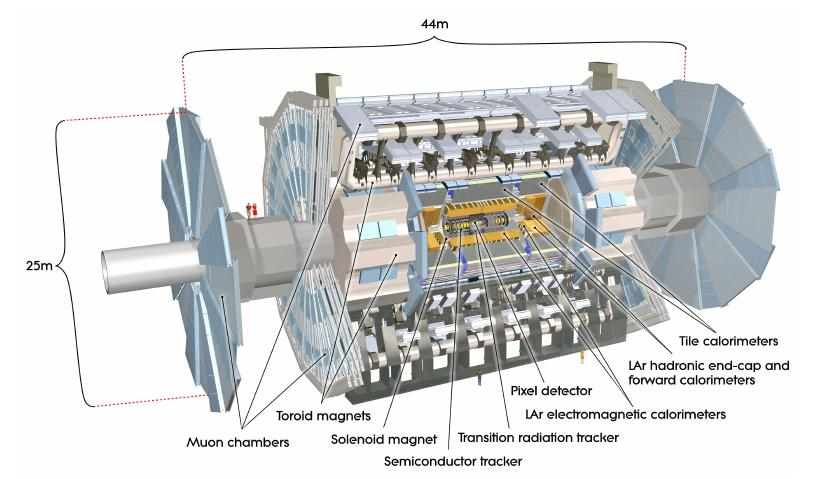
\includegraphics[width=11cm]{figures/atlas.jpg}
\caption{Cut-away view of the ATLAS detector with the different constituents.}
\label{ATLAS}
\end{figure}
There are four main parts the ATLAS detector consists of.
To begin with there is the inner detector which is the first component around the interaction point.
The task of the inner detector is the vertex resolution and furthermore the resolution of the momenta for all charged particles.
It consits of pixel and silicon microstrip detectors trackers and a Transition Radiation Tracker.
A solenoid magnet surrounds the inner detector and immerses it in a magnetic field. 
This causes the curvature of the charged particles tracks and ensures the momentum measurement.\\
The solenoid magnet is surrounded by the electromagnetic and hadronic calorimeters.
The electromagnetic calorimeter is further inside and makes precision measurements of electron and photon energies possible.
Electrons and photons ideally deposit all their energy in the electromagnetic calorimeter by interacting with the detector material.\\
The hadronic calorimeter performs the same goal as the electromagnetic calorimeter for hadrons, which are bound states of the quarks.
Hadrons form jets in the calorimeters.
The particles loose their energy because of hadronic showers in the hadronic calorimeter.
The outermost component of the ATLAS detector is the muon system or muon spectrometer.
For the ideal case only muons reach the muon spectrometer.
The muon spectrometer is immersed with a magnet field resulting from toroid magnets.
The magnets causes the deflection of the muons and enable momentum measurements as mentioned for the inner detector.




